
%(BEGIN_QUESTION)
% Copyright 2010, Tony R. Kuphaldt, released under the Creative Commons Attribution License (v 1.0)
% This means you may do almost anything with this work of mine, so long as you give me proper credit

Et DDC-system for byggautomasjon sender 4-20 mA styresignal til en dampventil med elektronisk posisjoner. Sløyfen har et problem: ventilen står helt stengt (0\%) uansett styring. En tekniker starter feilsøking med DC-spenningsmåling på klemrekke TB-10:

$$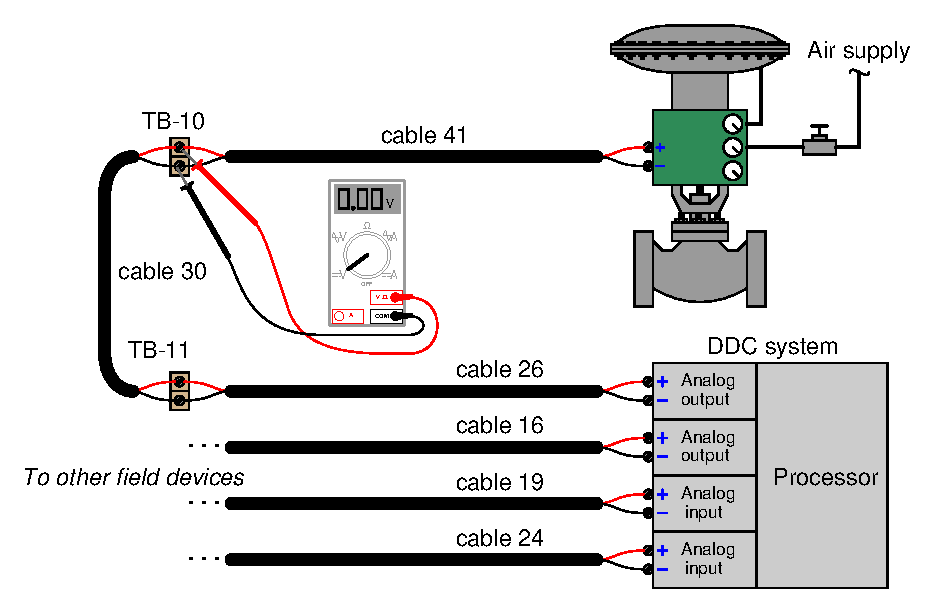
\includegraphics[width=15.5cm]{i00740x01.eps}$$

Teknikeren vet at 0 volt kan bety enten "åpen" feil eller "kortsluttet" feil i ledningene. Basert på målepunktet (0.00 VDC), angi hvor en enkelt åpen feil kan ligge (hvis det er årsaken), og hvor en kortslutningsfeil kan ligge (hvis det er årsaken).

\vskip 10pt

For neste test kobler teknikeren fra rød leder i kabel 41 på TB-10 og måler på nytt. Ny måling blir 24.9 volt. Bestem hva dette forteller om feiltype og feilsted.

\vskip 20pt \vbox{\hrule \hbox{\strut \vrule{} {\bf Forslag til sokratisk diskusjon} \vrule} \hrule}

\begin{itemize}
\item{} Forklar hvorfor det er kritisk å vite om ventil og DDC-kort er elektriske {\it kilder} eller {\it laster} når målinger tolkes.
\item{} Identifiser fordeler/ulemper med denne testmetoden (måle før/etter bevisst kabelbrudd) sammenlignet med andre multimetertester for å finne åpen/kortsluttet feil.
\item{} Identifiser en annen mulig feil enn åpen/kortsluttet kabel som kan forklare alle symptomer og målinger i scenariet.
\end{itemize}

\underbar{file i00740}
%(END_QUESTION)





%(BEGIN_ANSWER)

Basert kun på første måling kan vi konkludere at feilen {\it kan} være åpen feil i kabel 26 eller kabel 30, eller en kortslutning i {\it hvilken som helst} kabel.

%(END_ANSWER)





%(BEGIN_NOTES)

Etter andre måling må vi konkludere at feilen er en kortslutning (ikke åpen feil), og at den ligger et sted mellom TB-10 og reguleringsventilen (mest sannsynlig i kabel 41).

%INDEX% Feilsøking, repetisjon: elektriske kretser

%(END_NOTES)
